% dibuix_cilindre_1.tex
\documentclass{standalone}
\usepackage{tikz}
\usetikzlibrary{arrows.meta, decorations.markings}

\begin{document}

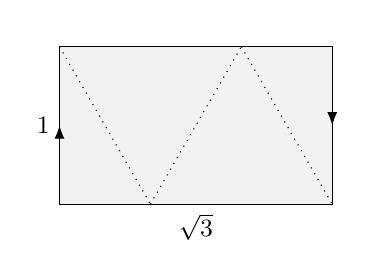
\begin{tikzpicture}[
    identified_edge/.style={
        decoration={
            markings,
            mark=at position 0.5 with {\arrow{Latex}}
        },
        postaction={decorate}
    },
    edge_label/.style={midway, auto, font=\small}
]

\def\squaresize{2}
\fill[gray!10] (0,0) -- (0,\squaresize) -- (1.73205080757 * \squaresize, \squaresize) -- (1.73205080757 * \squaresize,0) -- cycle;
\draw (0,0) rectangle (1.73205080757 * \squaresize,\squaresize);
\draw[black] (0,\squaresize) -- node[edge_label, above] {} (1.73205080757 * \squaresize,\squaresize);
\draw[black] (0,0)       -- node[edge_label, below]  {$\sqrt3$} (1.73205080757 * \squaresize,0);
\draw[identified_edge] (0,0)       -- node[edge_label, left]  {1} (0,\squaresize);
\draw[identified_edge] (1.73205080757 * \squaresize,\squaresize) -- node[edge_label, right] {} (1.73205080757 * \squaresize,0);
\draw[dotted] (0,\squaresize) -- node[edge_label, above] {} (1.73205080757 * \squaresize / 3,0);
\draw[dotted] (1.73205080757 * \squaresize / 3,0) -- node[edge_label, above] {} (2 * 1.73205080757 * \squaresize / 3,\squaresize);
\draw[dotted] (2 * 1.73205080757 * \squaresize / 3,\squaresize) -- node[edge_label, above] {} (1.73205080757 * \squaresize, 0);

\end{tikzpicture}

\end{document}